\documentclass[10pt]{article}

\usepackage[margin=1in, letterpaper]{geometry}
\usepackage{parskip}

\usepackage{amsthm, amsmath, amssymb}
% \usepackage{gensymb}  % For use of degree symbol
\usepackage[pdftex]{graphicx}
\usepackage{hyperref}

\usepackage{enumerate} % For use of (a), (b), et cetera
\usepackage{booktabs} % Tables
\usepackage[margin=10pt, labelfont=bf, labelsep=period,
justification=justified]{caption} % Captions in figure floats

% The following metadata will show up in the PDF properties
\hypersetup{
	colorlinks = true,
	urlcolor = blue,
	pdfauthor = {Aaron Tran},
	pdfkeywords = {x-ray, SNR, notes},
	pdftitle = {Supernova remnants and stuff - \today},
%	pdfsubject = {},
	pdfpagemode = UseNone
}

% Don't indent paragraphs
\setlength\parindent{0em}

% ===============
% Useful commands
% ===============
\newcommand{\mt}{\mathrm}
\newcommand{\unit}[1]{\; \mt{#1}} % vemod.net/typesetting-units-in-latex
\newcommand{\abt}{\mathord{\sim}} % tex.stackexchange.com/q/55701

\newcommand{\Chandra}{\textit{Chandra}}

\begin{document}

\begin{center}
    \Large{Some notes on SNRs}

    \normalsize
    Aaron Tran \\
    \today \\
\end{center}

These notes are assembled for my own self-edification, to learn about (1) X-ray
astronomy, both physics and observational pipeline, (2) supernovae and their
remnants, and (3) Tycho's SNR, and the physics relevant to my summer project.
Information comes from the literature, \Chandra\ info from the CXC, various
textbooks, and discussions with my mentors Brian Williams and Rob Petre.
Information may easily be wrong and I make no claims to accuracy/quality,
though I will aim to cite sources where possible.

This is a summer 2014 internship project under the auspices of GSFC and CRESST.
Mentors are Dr. Robert Petre and Dr. Brian J. Williams.

% =========
% Logistics
% =========
\section{GSFC logistics}

Notes from 1st meeting, Tues May 27.

Some things to attend.  July X-ray meeting to be moved.
\begin{itemize}
    \item 662 meeting -- 1st Friday of every month, 10:30am, Rm W120
    \item Coffee (just socializing) -- Weds 10am
    \item ASD colloquium -- Tues 3:45p (3:30p meet speaker), Rm W150
    \item GSFC colloquium -- Fri 3:30p, Bldg 3, Goett Auditorium
\end{itemize}

% ============
% Introduction
% ============
\section{Introduction}

A little bit about the project.  Builds on Ressler et al. (ApJ, in press).
Goal is to obtain FWHM of Tycho filaments.

If there is time, we will proceed to try perhaps Kepler, even Cas A (both are
quite a mess).  SN 1006 was HARDER than Tycho, really... so this is supposed to
be fairly straightforward!


% ===============
% X-ray astronomy
% ===============
\section{X-ray astronomy}

First, where are X-rays on the EM spectrum?  X-rays generally have energies
from $0.1$ to $100 \unit{keV}$.  They are divided into \emph{soft} and
\emph{hard} X-rays, where the division is at a few ($1$--$10$) keV.  Beyond
$\abt 100 \unit{keV}$ we move into gamma rays; below $\abt 0.1 \unit{keV}$ we
move back into ultraviolet.

Next, what emits X-rays?  What processes are probed?
X-ray emitting temperatures are about $10^6$ to $10^7$ K.
% TODO fill this in

Finally, what instruments conduct X-ray astronomy? The big ones are \Chandra,
\emph{XMM-Newton}, and \emph{Suzaku} (older ones incl. Einstein, ASCA, ROSAT).
Swift does have X-ray capability, but is designed for GRB detection; its X-ray,
UV, and optical imaging are for GRB afterglows.  It is also handy for transient
detection (e.g., if a nearby SN goes off...).  K. Dyer has put together a nice
\href{http://www.aoc.nrao.edu/~kdyer/useful/sat.html}
{table of past/present x-ray satellites}.

Nearby, NuSTAR is covering hard X-rays ($10$ to $100\unit{keV}$).  Fermi is
very far away, at $20\unit{MeV}$ to $\abt 50\unit{GeV}$.  In UV, the optical
astronomers kind of cover the near UV (e.g., HST).  GALEX, FUSE, EVUE also have
been flown but seem to be done?  Low end of extreme UV is $\abt 0.1\unit{keV}$.

Apparently, the tie between radio and X-ray observations is due to the imaging
of \emph{synchrotron radiation}?  So we can probe very energetic processes in
both bands.

% ---------
% Radiation
% ---------
\subsection{Radiative processes}

Synchrotron radiation, thermal (line) emission, etc.
% TODO study this


% =======
% Chandra
% =======
\section{\Chandra\ observations}

Our SNR observations are generally made with ACIS-I (occasionally ACIS-S).
ACIS has energy range about $0.7$ to $8 \unit{keV}$, see Figure \ref{fig:area}.
The suffixes (I,S) refer to the CCD array configuration, square for I and lined
up for S. No grating is used. Gratings would be used for spectroscopy --
perhaps HETG with ACIS-S (up to 1000 bins from $0.4$ to $10 \unit{keV}$).

How does ACIS work?  It's a CCD that enables photon counting, basically.
As Rob as noted, we get four pieces of information: time, energy, polarization,
and location on the sky.  We don't really care about time/polarization here
(since we are neglecting, or correcting for, proper motion).

The spectral resolution is frequency dependent (of course), but also \emph{row
number} dependent (i.e., depends on where on the CCD you strike).  The FWHM
resolution is around $100$--$300 \unit{keV}$, with decreasing resolution at
higher energy (FWHM scales as sqrt of energy); this assumes that a charge
transfer inefficiency correction is applied in CIAO.
Spectral resolution depends on how well we can measure the
energy deposited (in the form of mobilized charges, electron-hole pairs) by
each photon.  Apparently, the front-illuminated (FI) CCDs were damaged because
they were previously left in the focal plane during radiation belt passages.
So now they move it each time, which has minimized the damage!

\begin{figure}[!ht]
    \centering
    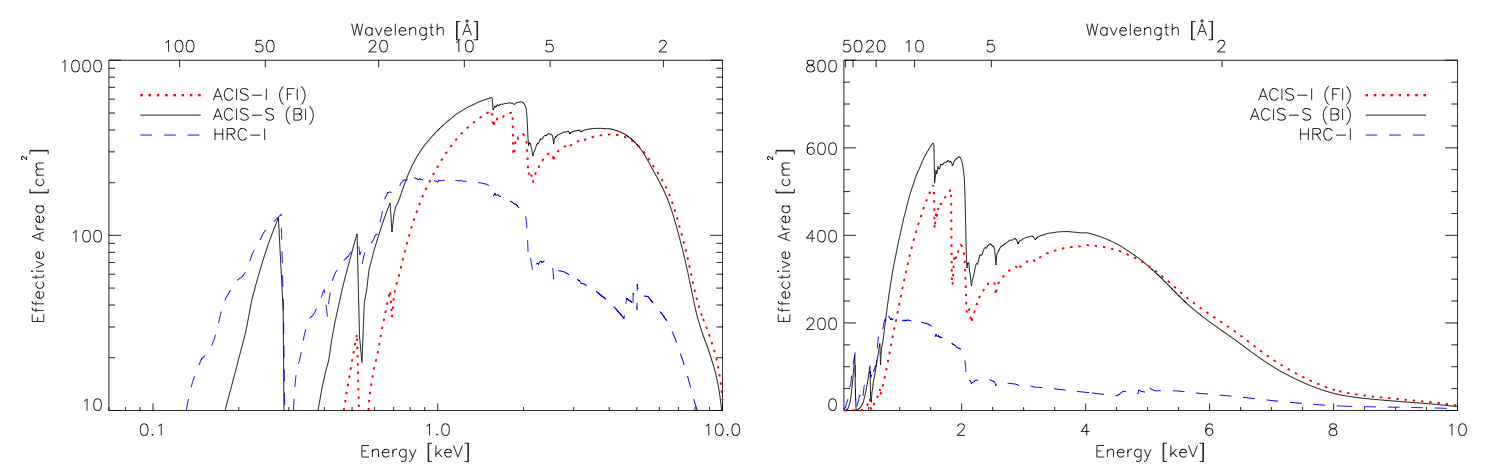
\includegraphics[width=\textwidth]{fig_chandra_area.png}
    \caption{On-axis effective areas for \Chandra\ instruments, predicted for
    Cycle 16 observations (2015?). Plot is for an integrated point source (?).
    Modified from \Chandra\ Cycle 16 POG, Figure 1.3.}
    \label{fig:area}
\end{figure}

Observations are broken into exposure chunks of $\abt10$ to $180 \unit{ksec}$,
limited by radiation belts and thermal considerations.

Information about specific observation runs are on \Chandra\
\href{http://cda.harvard.edu/chaser/}{WebChaSeR}
(simply search `Tycho' or `SN 1006').  Here you can get raw data, which can be
processed with CIAO and CALDB.
Information about the ACIS instrument is in
\href{http://cxc.harvard.edu/proposer/POG/html/chap6.html}{Chapter 6} of the
\href{http://cxc.harvard.edu/proposer/POG/html/index.html}{proposer's guide}.


% =================
% Supernova physics
% =================
\section{Supernova physics}
Velocities of forward
shock in supernovae are about $10^4$ km/s.  Very fast, very energetic.

About the ISM:
\href{notes}{http://ay201b.wordpress.com/2011/04/12/course-notes/}

% ===========
% Tycho's SNR
% ===========
\section{Tycho's SNR (SN 1572)}

Hayato et al., ApJ 2010, estimate
1. expansion velocity $\abt 4000$ to $5000 \unit{km/s}$, depending on which
spectral line you're looking at (Si, S, Ar faster than Fe K$\alpha$).
2. subsequently estimate Tycho's SNR to be $\abt 4 \unit{kpc}$ away from Earth

(I think this is still faster than usual ISM sound speed???)

For comparison, Sgr A* is $>8\unit{kpc}$ from Earth; the Milky Way is $\abt 34
\unit{kpc}$ across.  Andromeda is $\abt 780 \unit{kpc}$ away from us. (all this
from Wikipedia... just to give a sense of scale.  Our closest star (Proxima
Centauri) is about 1 parsec away.

Aliases: G120.1+1.4 Tycho, 3C10, SN1572
Bibliography on Tycho, up to 2009:
\href{Green's SNR catalogue}
{http://www.mrao.cam.ac.uk/surveys/snrs/snrs.G120.1+1.4.html}
Also more papers (up to 2014) \href{here}
{http://www.physics.umanitoba.ca/snr/SNRcat/SNRrecord.php?id=G120.1p01.4}

Acciari et al. 2011 ApJL, find TeV gamma rays in a smush, around the SNR
BEAUTIFUL picture of a CO cloud possibly interacting, and the gamma ray
emissions is offset as well.  Short, sweet paper.

Giordano et al. 2012 ApJ, Fermi LAT observation of Tycho.
Describe emission as due to pion decays from cosmic-ray acceleration into ISM.
\href{iop}{http://iopscience.iop.org/2041-8205/744/1/L2/}

B field amplification (2004)
\href{arxiv}{http://arxiv.org/pdf/astro-ph/0409453v2.pdf}
(Tycho and similar)
Nonthermal filaments study (2005)
\href{iop}{http://iopscience.iop.org/0004-637X/621/2/793/pdf/0004-637X\_621\_2\_793.pdf}

\subsection{SN 1006}


%\begin{table}[t]
%\centering
%\caption{Comparison of predicted and observed frequency aliasing.
%Predicted uncertainties are estimated from maximum observed fluctuation in
%oscilloscope measurements of signal period; we are unable to estimate and
%include error in sampling frequency.
%Observed uncertainty is set to frequency resolution $\sim 10 \unit{kHZ}$, set
%by discrete Fourier transform (number of samples and sample rate).}
%\begin{tabular}{@{}rrr@{}}
%    \toprule
%    & \multicolumn{2}{c}{$f_{\mt{aliased}} \unit{(MHz)}$} \\
%    \cmidrule(l){2-3}
%    $f_{\mt{sig}} \unit{(MHz)}$ & predicted & observed \\
%    \midrule
%    0.88 & $0.88 \pm 0.003$ & $0.87 \pm 0.01$ \\
%    3.52 & $3.52 \pm 0.02$ & $3.52 \pm 0.01$ \\
%    6.16 & $3.84 \pm 0.08$ & $3.83 \pm 0.01$ \\
%    7.92 & $2.08 \pm 0.04$ & $2.09 \pm 0.01$ \\
%    8.80 & $1.20 \pm 0.03$ & $1.21 \pm 0.01$ \\
%    26.4 & $3.60 \pm 0.3$ & $3.61 \pm 0.01$ \\
%    \bottomrule
%\end{tabular}
%\end{table}

\end{document}
